	\documentclass[twoside]{article}
\usepackage{../estilo-ejercicios}
%\renewcommand{\baselinestretch}{1,3}
%--------------------------------------------------------
\begin{document}

\title{Ejercicios de Modelado y Simulación Topológica}
\author{Javier Aguilar Martín}
\maketitle
En los diagramas de persistencia, la barra diagonal no es representativa, solo indica la bisectriz del cuadrante
\begin{ejercicio}{4}
\end{ejercicio}
\begin{solucion}
Complejo hecho en geogebra por la profesora, debe de subirlo a la ev. 
\end{solucion}
\newpage

\begin{ejercicio}{5}
\end{ejercicio}
\begin{solucion}
Es largísimo de hacer porque son muchos pasos. No depende del orden, se puede ir viendo por casos (es bastante ilustrativo para las componentes conexas)
\end{solucion}

\newpage

\begin{ejercicio}{6}
Dibuja los diagramas de persistencia y los códigos de barras de la siguiente filtración:
\begin{figure}[h!]
\centering
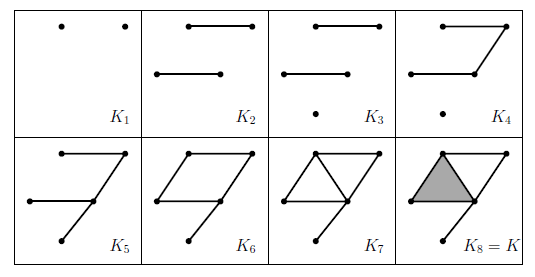
\includegraphics[scale=0.8]{1-6}
\end{figure}
\end{ejercicio}
\begin{solucion}
Para $p=0$ una componente $\gamma_1$ nace en 1 y va hasta el infinito (correspondiente a uno cualquiera de los puntos), $\gamma_2$ nace en 1 y muere en 2 (correspondiente al otro punto), otra componente $\gamma_3$ nace en 2 y muere en 4 (el segmento inferior), $\gamma_4$ nace en 3 y muere en 5 (el último vértice aislado). En persistencia esto da solo una recta horizontal y varios puntos por encima de la bisectriz.

Para $p=1$ tenemos $\gamma_1$ que nace en 6 y va hasta el infinito, o sea hasta 8 y $\gamma_2$, que nace en 7 y muere en 8. En persistencia esto da una recta horizontal y el punto $(7,8)$. 
\end{solucion}

\newpage

\begin{ejercicio}{7}
Sea $K$ un complejo simplicial abstracto de dimensión 1 en el que cada vértice es cara de a lo
sumo dos 1-símplices. ¿Se puede dar una realización geométrica de $K$ en el plano en la que
para cada 1-símplice sus dos vértices extremos estén a la misma distancia? En tal caso, ¿cómo
sería la filtración por complejos alfa?
\end{ejercicio}
\begin{solucion}
Como cada vértice tiene a lo sumo grado 2, el resultado es un camino $P_n$ o un ciclo $C_n$, donde $n$ es el número de vértices, que se pueden hacer con sus aristas de la misma longitud. Recordar que los complejos alfa salen de considerar el diagrama de Voronoi y hacer bolas alrededor de los puntos que se van agrandando hasta chocar con el borde de las celdas de Voronoi, después de eso, solo aumentan por donde no hayan chocado. Cada choche con un borde genera un símplice de dimensión el número de celdas que compartan borde menos 1. A partir de eso es fácil.
\end{solucion}

\end{document}
